% !TEX root = DesignDocument.tex

\chapter{User Stories,  Requirements, and Product Backlog}
\section{Overview}

This document contains the features, creation and develpment of crowd control. It covers prerequsit user stories, to the design and implimentation of the application its self.

%The overview should take the form of an executive summary.  Give the reader a feel 
%for the purpose of the document, what is contained in the document, and an idea 
%of the purpose for the system or product. 

 %The user stories 
%are provided by the stakeholders.  You will create he backlogs and the requirements, and document here.  
%This chapter should contain 
%details about each of the requirements and how the requirements are or will be 
%satisfied in the design and implementation of the system.

%Below:   list, describe, and define the requirements in this chapter.  
%There could be any number of sub-sections to help provide the necessary level of 
%detail. 




\section{User Stories}
%This section can really be seen as the guts of the document.  This section should 
%be the result of discussions with the stakeholders with regard to the actual functional 
%requirements of the software.  It is the user stories that will be used in the 
%work breakdown structure to build tasks to fill the product backlog for implementation 
%through the sprints.

%This section should contain sub-sections to define and potentially provide a breakdown 
%of larger user stories into smaller user stories.   Each component must have a test identified, 
%meaning you need to know how you plan to test it.  If a requirement is not testable, then 
%some justification needs to be made on why the requirement has been included.  
 %The results of the tests should go in the testing chapter. 


\subsection{User Story \#1 }
As a user I want to join a public group.

\subsubsection{User Story \#1 Breakdown}
The user can request to join any public group.  Their request will be sent to the group leader for approval.  Depending on the group leaders action then the user will be accepted or denied access to the group. 

\subsection{User Story \#2 }
As a user i want to be able to join a private group.

\subsubsection{User Story \#2 Breakdown}
For the user to join a private group they must first recieve an invitation from the group leader of the private group of interest.  Then the user can either accept or reject the invitation to join the group.  If the invitation is accepted then the user is placed into the group and then starts sharing information. 

\subsection{User Story \#02} 
As a user i want to see other group members on a map

\subsubsection{User Story \#02 Breakdown}
Once the user is in a group then the user will have access to a map that displays the locations of all users that are members of the group.

\subsection{User Story \#3} 
As a user i want post agenda for the group.

\subsection{User Story \#4} 
As a user i want to see a list of public groups nearby

\subsection{User Story \#5} 
As a user i want the ability to have suggestions of local activities.

\subsection{User Story \#6} 
As a user i want the ability to leave a group.

\subsection{User Story \#7} 
As a user i want the ability to have a list of local groups.

\subsection{User Story \#8} 
As a user i want the abilitiy to login.

\subsection{User Story \#9}
As a user i would like to message other members of the group.

\subsection{User Story \#10} 
As a user i would like my information protected. 




\section{Requirements and Design Constraints}
%Use this section to discuss what requirements exist that deal with meeting the 
%business need.  These requirements might equate to design constraints which can 
%take the form of system, network, and/or user constraints.  Examples:  Windows 
%Server only, iOS only, slow network constraints, or no offline, local storage capabilities. 

This section will cover the main design requirement in all aspects of crowd control.


\subsection{System  Requirements}
%What are they?  How will they impact the potential design?  Are there alternatives? 

Sense there we are creating Crowd Control to run on two different platforms, both iOS and Android, there are two sets of requirements that will be similar between both platforms. Even though they are both similar, implimentation between both will be differnet. With them both being different they are split into two sections as listed below.

\subsubsection{iOS Requirements}
\begin{itemize}
\item{Use Apple Mapping Features}
\item{Access Parse as the Database}
\end{itemize}
\subsubsection{Android Requirements}
\begin{itemize}
\item{Use Google Maps}
\item{Access Parse as the Database}
\end{itemize}
\subsubsection{Parse Requirements}
\begin{itemize}
\item{Delete groups when group is not in use}
\end{itemize}

\subsection{Network Requirements}
%What are they? 

Network requrements are mobile networks as this is a mobile applications. The requirement on our part is making sure that the application is able to reach the server and use at little data as possible when connected to the network. Making sure we use as little data as possible will help our users not use all of their data. 

\subsection{Development Environment Requirements}
%What are they?  Is the system supposed to be cross-platform?

The development enviroment requirement is that Crowd Control be avalabe on both iOS and Android platforms. Being cross platform allows for us to reach as many users as possible. Android development will be handled with Android Studio and iOS will be developed with xCode.


\subsection{Project  Management Methodology}
%The stakeholders might restrict how the project implementation will be managed. 
 %There may be constraints on when design meetings will take place.  There might 
%be restrictions on how often progress reports need to be provided and to whom. 

We have set restrictions on the developemnt of Crowd Control and are listed as follows:
 
\begin{itemize}
\item GitHub issues will be used to keep track of current status as well as backlogs for the product.
\item There will be 6 total sprints over 2 scimesters for this products.
\item The sprint cycles are 3 weeks long.
\item Progress reports will be summited to Dr. McGough and Brian Butterfeild at the end of each sprint.
\item Github will be used for source control. 
\end{itemize}


\section{Specifications}
%Any specifications that need to be understood?  Put it here.  

\section{Product Backlog}
%The full product backlog should go here.  The sprint backlogs are located in the project chapter.

 
\begin{itemize}
\item What system will be used to keep track of the backlogs and sprint status?
\item Will all parties have access to the Sprint and Product Backlogs?
\item How many Sprints will encompass this particular project?
\item How long are the Sprint Cycles?
\item Are there restrictions on source control? 
\end{itemize}


\section{Research or Proof of Concept Results}
%This section is reserved for the discussion centered on any research that needed 
%to take place before full system design.  The research efforts may have led to 
%the need to actually provide a proof of concept for approval by the stakeholders. 
 %The proof of concept might even go to the extent of a user interface design or 
%mockups. 


The Proof of conecpt is a rough design that impliments basic features of Crowd Control. Basic features are currently under construction. This is currently a functional prototype with improvements in the future.
\newline 
\newline
Below are screen shots of both android and iOS proof of concepts.
(current formatting issues need to fix)
\subsection{iOS Proof of Concept Screen Shots}

Below are screen shots from the iOS version of CrowdControl.


	\begin{figure}[tbh]
	\begin{center}
	\fbox{\includegraphics[scale=.1 ]{Additional/iOS/iOSPictures/img_3901.png}}
	\end{center}
	\caption{iOS login select screen \label{iOSloginselectscreen}}
	\end{figure}

	\begin{figure}[tbh]
	\begin{center}
	\fbox{\includegraphics[scale=.1]{Additional/iOS/iOSPictures/img_3896.png}}
	\end{center}
	\caption{iOS email login screen \label{iOSemailLoginScreen}}
	\end{figure}

	\begin{figure}[tbh]
	\begin{center}
	\fbox{\includegraphics[scale=.1]{Additional/iOS/iOSPictures/img_3897.png}}
	\end{center}
	\caption{iOS create account screen \label{iOScreateAccountScreen}}
	\end{figure}

	\begin{figure}[tbh]
	\begin{center}
	\fbox{\includegraphics[scale=.1]{Additional/iOS/iOSPictures/img_3898.png}}
	\end{center}
	\caption{iOS group infomation screen \label{iOSGroupScreen}}
	\end{figure}

	\begin{figure}[tbh]
	\begin{center}
	\fbox{\includegraphics[scale=.2]{Additional/iOS/iOSPictures/img_3899.png}}
	\end{center}
	\caption{iOS map view screen \label{iOSmapScreen}}
	\end{figure}

	\begin{figure}[tbh]
	\begin{center}
	\fbox{\includegraphics[scale=.1]{Additional/iOS/iOSPictures/img_3900.png}}
	\end{center}
	\caption{iOS messaging main screen \label{iOSmessagingMain}}
	\end{figure}


\subsection{Android  Proof of Concept Screen Shots}

Below are screen shots from the Android version of CrowdControl.


	\begin{figure}[tbh]
	\begin{center}
	\fbox{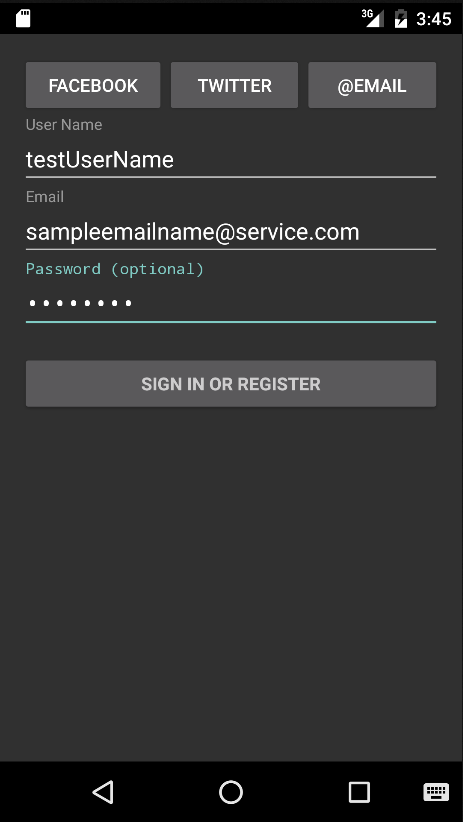
\includegraphics[scale=.4]{Additional/Android/AndroidPictures/loginScreen.png}}
	\end{center}
	\caption{Android login screen \label{AndroudLoginScreen}}
	\end{figure}

	\begin{figure}[tbh]
	\begin{center}
	\fbox{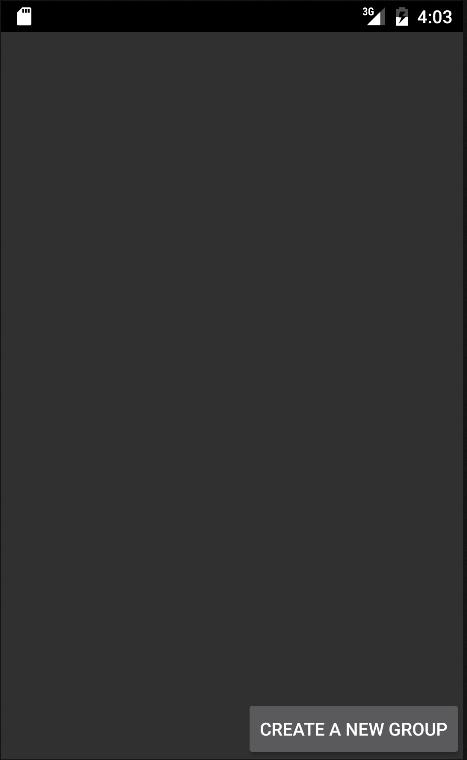
\includegraphics[scale=.4]{Additional/Android/AndroidPictures/createNewGroup.png}}
	\end{center}
	\caption{Android create group screen \label{AndroidCreateGroup}}
	\end{figure}

	\begin{figure}[tbh]
	\begin{center}
	\fbox{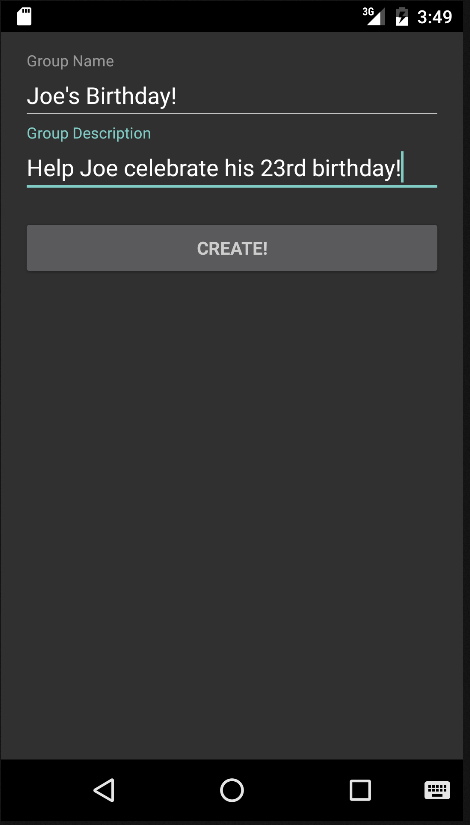
\includegraphics[scale=.4]{Additional/Android/AndroidPictures/groupCreatePage.png}}
	\end{center}
	\caption{Android group information screen \label{AndroidGroupInfo}}
	\end{figure}

	\begin{figure}[tbh]
	\begin{center}
	\fbox{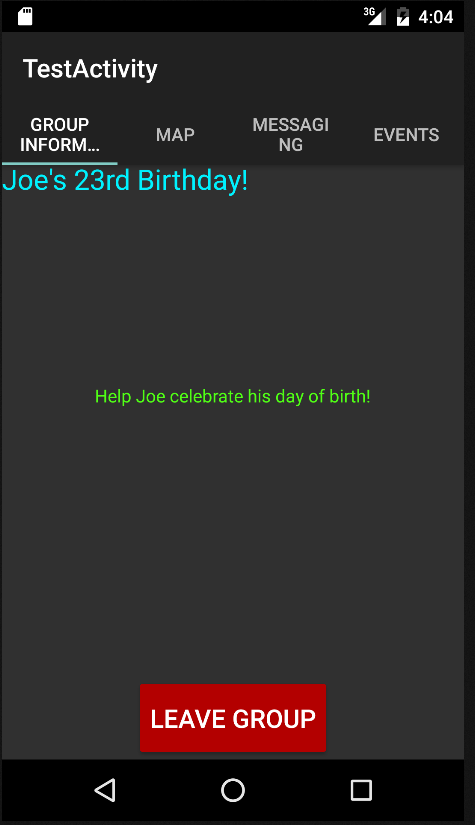
\includegraphics[scale=.4]{Additional/Android/AndroidPictures/groupJoinedPage.png}}
	\end{center}
	\caption{Android group join screen \label{AndroidJoinGroup}}
	\end{figure}

	\begin{figure}[tbh]
	\begin{center}
	\fbox{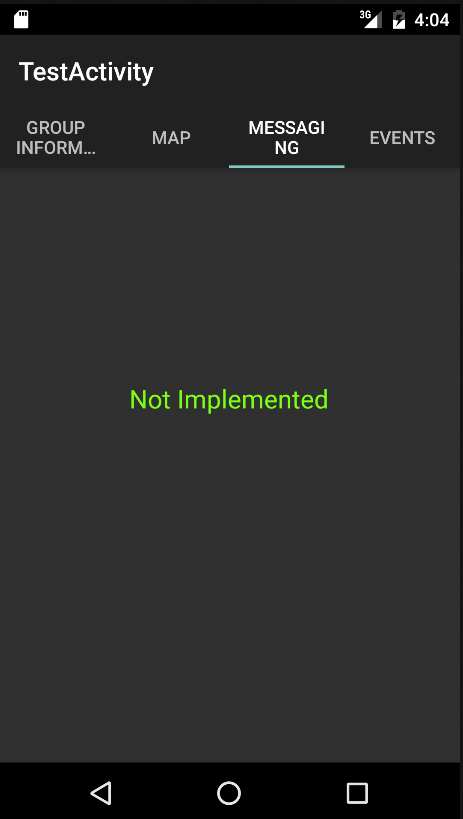
\includegraphics[scale=.4]{Additional/Android/AndroidPictures/messagingNotImplemented.png}}
	\end{center}
	\caption{Android messaging main screen \label{AndroidMessagingMain}}
	\end{figure}


\section{Supporting Material}


%This document might contain references or supporting material which should be documented 
%and discussed  either here if appropriate or more often in the appendices at the end.  This material may have been provided by the stakeholders  
%or it may be material garnered from research tasks.

